\chapter{Optical Sensors and Object Detection}
\label{ch:Optical Sensors and Object Detection}

\section{Introduction}
The detection of light from the light sources intuits the idea of vision, based on what the human eyes are working on. When light strikes on any object, some part of it is absorbed by the object, and the rest is reflected into the environment. This reflected part makes its way to the human eyes and accumulates on the retina. The light collected in the retina generates a picture of the object from where it is reflected. This kind of natural phenomenon has immense importance in the development of photosensitive instruments \cite{opencv} and such devices are widely used in the computer vision field. It is a multidisciplinary scientific field that primarily deals with a high-level understanding of the images, which is used to extract numerical and symbolic information of the scene. Further, this information is used to make a useful decision in autonomous robotic applications.

Object detection is a computer vision technique that uses to locate an object within an image or video frame. The primary goal of object detection is to replicate human intelligence using a computer. Object detection algorithms use many machine learning techniques such as convolutional neural networks, image thresholding, RGB color channel segmentation, support vector machines, and aggregate channel features.
    
\section{Optical Sensor: Camera}
A camera is a small sealed box with light-sensitive film in it. A small hole on the box is positioned in such a way that it allows limited light rays that concentrate at a single point. This point is known as an optical center, and the distance between the optical center and photographic film is known as focal length. Such a camera cannot be used for practical purposes since its light detection capacity is very small. Therefore, it is equipped with an external lens to increase the light gathering capacity. Two types of camera sensor arrays are used in an autonomous robotic application: 1. Single pinhole camera and 2. Stereo camera. These will be discussed in detail further in the following section.

\subsection{Single Pin-hole Camera}
A simple geometric arrangement of a single pin-hole camera is illustrated in Fig. \ref{pinhole}. A reflected light ray from the object Q located at $(X, Y, Z)$ passes through the image plane and heads towards the center of projection or optical center, and q$(x,y,f)$  is the object's projection on the image plane. The object's position is defined in the world frame, which is a Cartesian coordinate system. While, the object's projection is defined in the image frame, which is a homogeneous coordinate system. The simple projective transformation from world frame to image frame by use of similar triangles is as follows.
 
\begin{equation}
x =  \frac{f \cdot X}{Z} , y = \frac{f \cdot Y}{Z} 
\label{eq21}
\end{equation}

Where, f is the focal length of the camera. 
 
Three reference frames used to illustrate the camera model are: (1) World Frame, (2) Camera Frame, and (3) Image Frame. The parameters used to describe the transformation from world coordinates to camera coordinates are called extrinsic. And those from camera coordinates to image coordinates are called intrinsic. Extrinsic parameters represent the 3-D Euclidean transformation between the world frame and camera frame. And intrinsic parameters represent projective or homogeneous transformation between 3-D camera frame and 2-D image frame. The camera model derived using intrinsic and extrinsic parameters is mentioned below.       

\begin{figure}
    \centering
    \fbox { 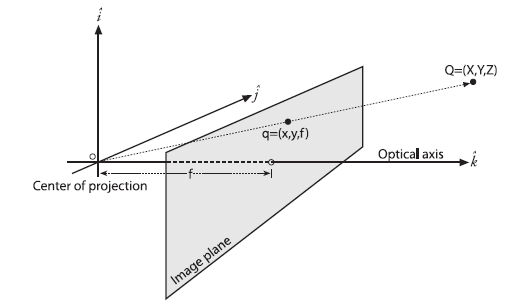
\includegraphics[scale= 0.8]{Images/pinhole.png}}
    \caption{Single Pin-hole Camera Model \cite{opencv}}
    \label{pinhole}
\end{figure}

\begin{equation}
\left[\begin{array}{ccc}
x \\
y \\
1
\end{array}\right] 
 = K \times 
\left[\begin{array}{ccc}
R & t
\end{array}\right] 
 \times
\left[\begin{array}{ccc}
X \\
Y \\
Z \\
1
\end{array}\right]  
\end{equation}

\begin{equation}
K = \left[\begin{array}{ccc}f_{x} & 0 & 0 \\ s & f_{y} & 0 \\ c_{x} & c_{y} & 1\end{array}\right] 
\end{equation}

Where, K is a intrinsic matrix, R and t are rotation and translation matrices, $(f_{x},f_{y})$ is a focal length in pixel, $(c_{x},c_{y})$ is optical center coordinates in pixel, and s is skew coefficient. 

\subsection{Stereo Vision}
A stereo camera is composed of two cameras situated in a tandem way with a small distance between them. It is mainly used to simulate human binocular vision. By looking at the single object from two different positions, the object's location appears different concerning two individual camera's image frames. This difference is known as disparity which can be used to compute 3D world coordinates of the object by using triangulation. Stereo imaging requires four steps to accurately estimate the depth data: 1. Undistortion, 2. Rectification, 3. Correspondence Formation, and 4. Triangulation.

\textbf{1. Undistortion:}
The cameras are used with external wide view lenses that result in image distortion. There are two types of distortions: Radial and tangential. The image can be undistorted by using radial and tangential distortion models. Light rays at the edge of a lens bend much more compare to rays close to the lens optical center which results in radial distortion. Due to radial distortion, the straight edge of any object appears curved in the image as seen in Fig. \ref{radial}. Radial distortion is modeled using radial distortion coefficients of the lens as shown in Eq. (\ref{radialdistortion}).

\begin{equation}
\begin{array}{l}
x_{\text {distorted }}=x\left(1+k_{1} \cdot r^{2}+k_{2} \cdot r^{4}+k_{3} \cdot r^{6}\right) \\
y_{\text {distorted }}=y\left(1+k_{1} \cdot r^{2}+k_{2}{ } \cdot r^{4}+k_{3}{ } \cdot r^{6}\right)
\end{array}
\label{radialdistortion}
\end{equation}

Where, x and y are undistorted normalized pixel coordinates, $k_{1}, k_{2},$ and $k_{3}$ are radial distortion coefficients, and r is the radial distance from the optical center.  

\begin{figure}
    \centering
    \fbox { 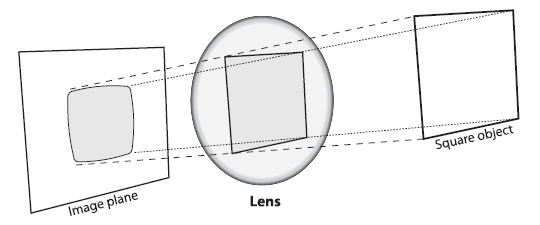
\includegraphics[scale=0.8]{Images/radial.png}}
    \caption{Radial Distortion \cite{opencv}}
    \label{radial}
\end{figure}

Tangential distortion occurs when the lens plane is not completely parallel with the image plane as seen in Fig. \ref{tangential}. This may happen due to manufacturing defect or use of cheap glue to stick the imager in the camera. It is modelled using tangential distortion coefficients of the lens as shown in Eq. (\ref{tengetialdistortion}).

\begin{equation}
\begin{array}{l}
x_{\text {distorted }}=x+\left[2 \cdot p_{1} \cdot x \cdot y+p_{2} \cdot \left(r^{2}+2 \cdot x^{2}\right)\right] \\
y_{\text {distorted }}=y+\left[p_{1} \cdot\left(r^{2}+2 \cdot y^{2}\right)+2 \cdot p_{2} \cdot x \cdot y\right]
\end{array}
\label{tengetialdistortion}
\end{equation}

Where, x and y are undistorted normalized pixel coordinates, $p_{1}$,and $p_{2}$ are tangential distortion coefficients, and r is the radial distance from the optical center. 

\begin{figure}
    \centering
    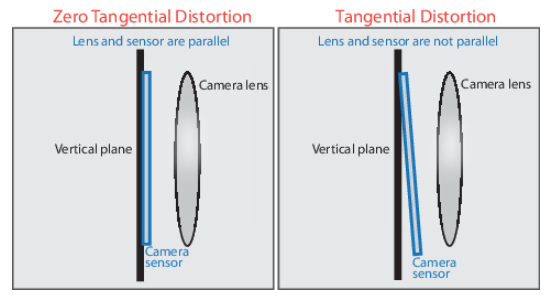
\includegraphics[scale= 0.7]{Images/tangential.png}
    \caption{Tangential Distortion \cite{MATLAB_camera}}
    \label{tangential}
\end{figure}

\textbf{2. Rectification:}
Rectification is the process in which images from two camera sensors are rotated and twisted to make the difference between their y coordinates to zero. Firstly, any point of interest is multiplied with an essential or fundamental metric which is derived in stereo camera intrinsic calibration to find its corresponding epipolar line in another view. These two epipolar lines from both the views are then made parallel to the horizontal axis of the stereo camera. Image rectification is performed when two cameras are not aligned and their image planes are not co-planner. This is usually the case for all manufactured stereo cameras because it is very difficult to maintain perfect coplanarity between two cameras.   

\textbf{3. Correspondence Formation:}
In this step, a search algorithm is used that finds similar features in both images. This is a computationally expensive process. However, prior knowledge of the object geometry can be helpful to reduce the search space. The result of this step is a disparity map, where the value of disparity is a difference in x - coordinates of corresponding points in the images from left and right cameras. 

\textbf{4. Triangulation:}
Triangulation is a technique where the depth information is derived by the use of prior knowledge of disparity and distance between two cameras. As shown in Fig. \ref{triangulate}, the depth information is easily computed by the use of a similar triangle rule. The relationship between depth and disparity is shown in Eq. (\ref{triangulation}).

\begin{equation}
Z = \frac{f \cdot T}{x^l - x^r}
\label{triangulation}
\end{equation}

Where, Z is a depth of object w.r.t stereo camera, f is a focal length, T is a horizontal distance between two cameras, and $x^l$ and $x^r$ are the projection of object P on the left camera image plane and right camera image plane respectively. 

It can be inferred from the above equation that the depth is inversely proportional to the disparity. The error in-depth calculation increases as the disparity value get closer to zero. Therefore, the depth resolution is precise only for the objects which are relatively near to stereo camera than distant objects. 

\begin{figure}
    \centering
    \fbox { 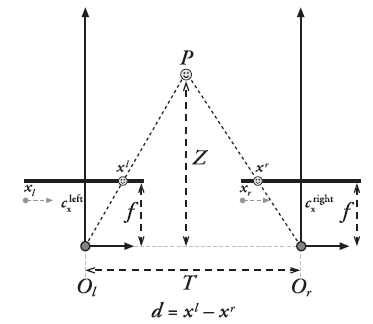
\includegraphics[scale= 0.7]{Images/triangulate.png}}
    \caption{Triangulation \cite{opencv}}
    \label{triangulate}
\end{figure}

\subsection{Sony IMX 179 sensor features}
This work uses two Sony IMX 179 image sensors for stereo vision. This sensor is accompanied by a non-distortion lens which has a $75^o$ field of view in a horizontal direction. The features of this sensor are mention below.

\begin{itemize}
\item CMOS active pixel type dots
\item CSI2 serial data output
\item RGB primary color pigment mosaic filters on chip
\item Max. 30 fps in all pixel scan mode
\item 8 MP high definition resolution 
\item Image Resolutions available: 3264 X 2448, 3200 X 2400, 1024 X 768
\end{itemize}

\begin{figure}
    \centering
    \fbox { 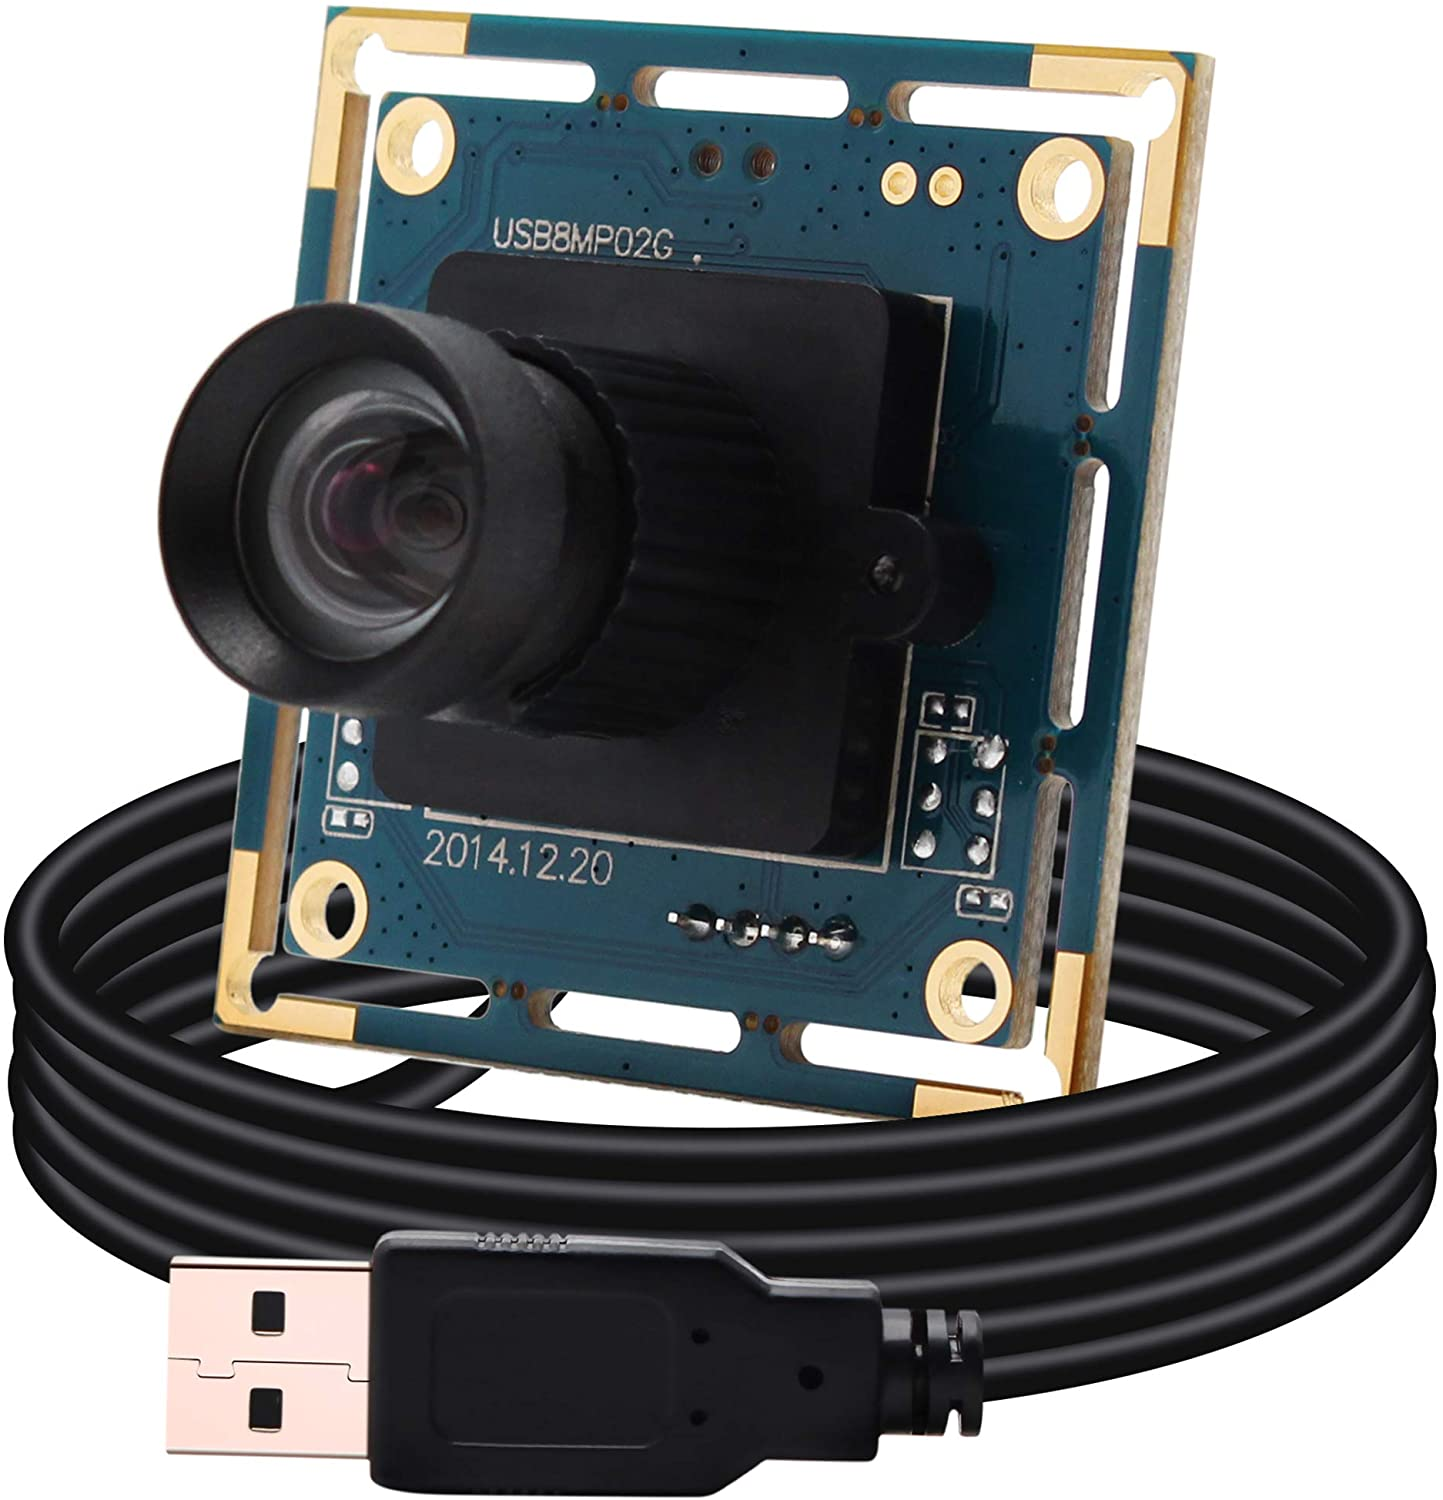
\includegraphics[scale= 0.15]{Images/imx179.png}}
    \caption{Sony IMX 179 Image Sensor with Non-Distortion Lens}
    \label{imx179}
\end{figure}

\section{Optical Sensor: 3-D LiDAR Camera}
LiDAR stands for Light Detection And Ranging. It is one of the remote sensing methods that uses a pulsing laser to measure the range of an object. LiDAR instruments were initially used for terrain mapping, surveying and are fitted on satellites and aircraft. However, in recent years it is widely used in autonomous driving applications. It works on the principle of time of flight. The range resolution of LiDAR can be defined by Eq. (\ref{Lidarrange}). LiDAR generates the object's data in form of a point cloud which is composed of X, Y, Z range channels, Intensity, and RGB channels. A LiDAR scanner is a type of instrument that rotates around its axis to scan the surroundings. However, in this research work, a LiDAR camera is used, which has $70^o$ of the horizontal field of view, to get 3D point cloud data.            

\begin{equation}
R = \frac{c}{2 B}
\label{Lidarrange}
\end{equation}

Where, R is a range, c is a speed of light in the corresponding medium, and B is the system bandwidth.

\begin{figure}
    \centering
    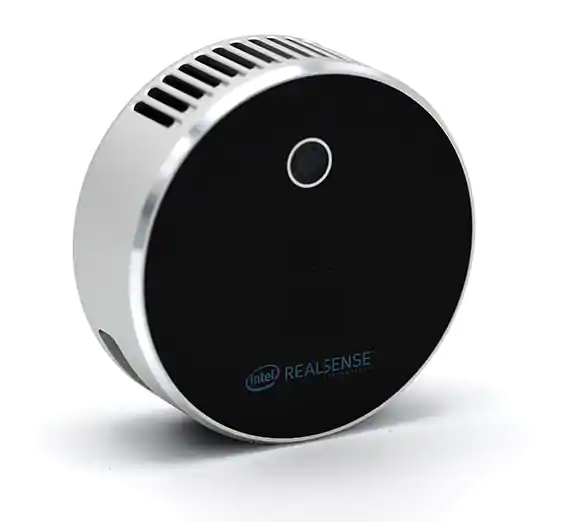
\includegraphics[scale= 0.5]{Images/L515.png}
    \caption{Intel Realsense LiDAR Camera L515}
    \label{L515}
\end{figure}

\subsection{Intel Realsense L515}
The Intel Realsense LiDAR camera L515 is the first camera manufactured by Intel that enables high-resolution accurate depth sensing. It is designed specifically to be used in a remote-controlled mobile robotics application. Some features of this LiDAR instrument are mention below.

\begin{itemize}
\item Depth capture at 95 percent reflectively of surface is 0.25 m to 9 m
\item Diameter is 61 mm and height is 26 mm
\item Approximate Weight is 100 g
\item Power consumption is 3.5 W
\item A short exposure time of laser is less than 100 ns per depth point
\item A number of depth points per second is 9.2 M at 640 X 480 and 23.6 M at 1024 X 768 image resolution
\item Depth accuracy is 5 mm to 14 mm
\end{itemize}

\section{Sensor Calibration}
The formal definition of calibration is "Operation that, under specified conditions, in a first step, establishes a relation between the quantity values with measurement uncertainties provided by measurement standards and corresponding indications with associated measurement uncertainties (of the calibrated instrument or secondary standard) and, in a second step, uses this information to establish a relation for obtaining a measurement result from an indication"\cite{calibration}.

It is clearly stated in the definition that the calibration process is completely based on the comparison. In the calibration process, two datasets are used which are the ground truth and sensor measurement dataset. Ground truth dataset is precisely generated using standard measurement instrument while measurement data is collected from the sensor which is going to calibrate. By re-projecting, the measurement data on ground truth data, the standard error of the respective sensor can be derived.     

No sensor is 100 percent accurate. Thus, the calibration of sensors is an essential part of the system. The calibration is done to find standard measurement error is called intrinsic calibration whereas the calibration is done to find standard transformation error between two measurement sensors is called extrinsic calibration.

\subsection{Stereo Camera Intrinsic Calibration}
Intrinsic camera parameters are calculated by first taking forty images of checkered board patterns at different positions w.r.t to the camera. Five images out of forty were ignored because of the high reprojection error. Further, the calibration was performed which has 0.37 pixels of re-projection error as shown in Fig. \ref{camintrinsic1}. The histogram of standard measurement error of stereo camera is shown in Fig. \ref{camintrinsic2} and standard measurement error is also mentioned in table \ref{Intrinsics}.      

\begin{table}
    \centering
    \begin{tabular}{|l|c|c|}
        \hline
        Description & Stereo Camera & LiDAR \\
        \hline
        X Error & 0.08 mm & 0.10 mm \\
        \hline
        Y Error & -0.09 mm & -0.04 mm \\ 
        \hline
        Z Error & -0.03 mm  & -0.19 mm \\
        \hline
        Overall Error & -4.5 mm & -21.89 mm \\
        \hline
    \end{tabular}
    \caption{Measurement Error of Intrinsic Calibration}
    \label{Intrinsics}
\end{table}

\begin{figure}
    \centering
    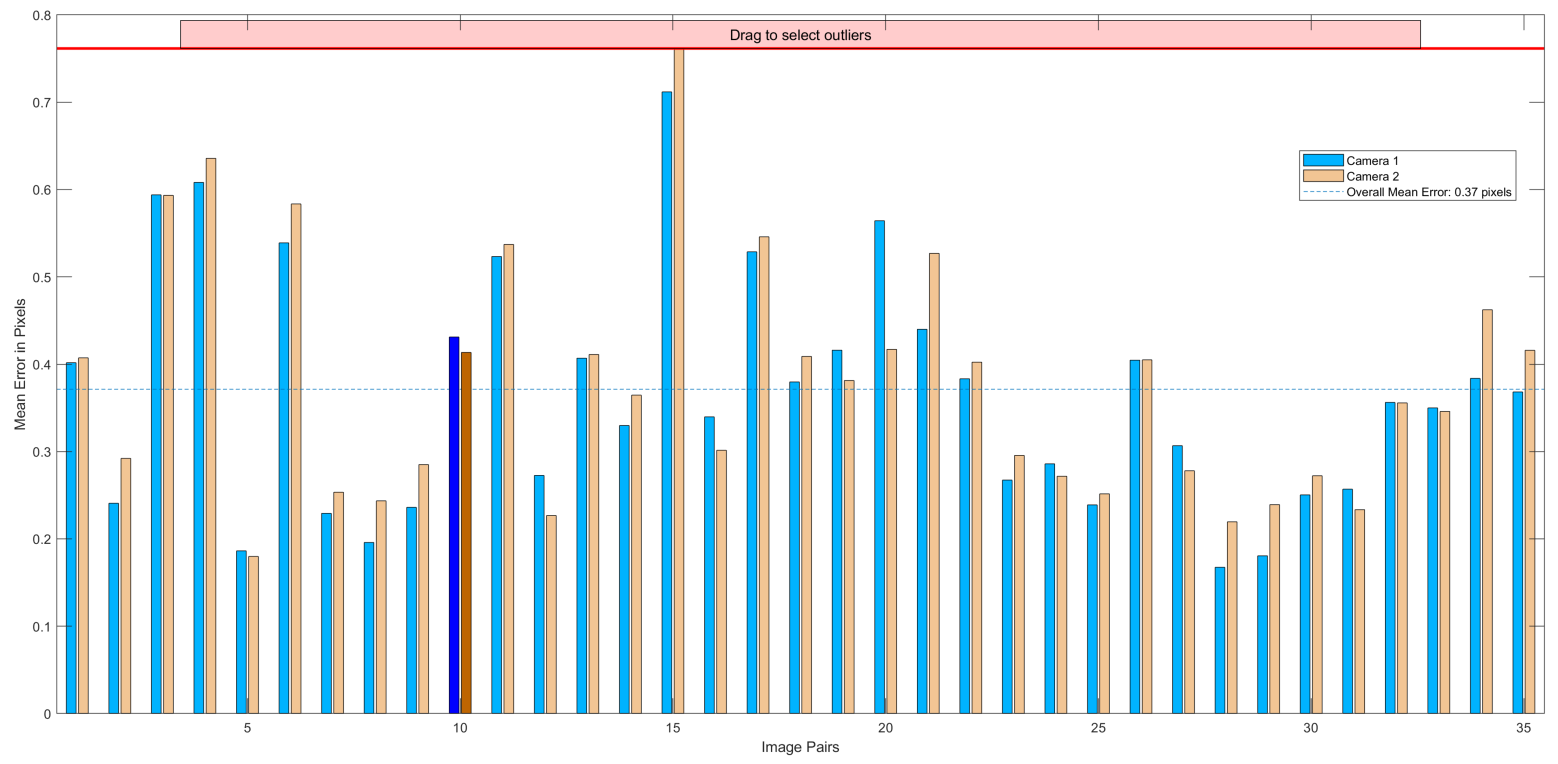
\includegraphics[scale= 0.27]{Images/camintrinsic1.png}
    \caption{Camera Intrinsic Calibration to find Intrinsic parameters}
    \label{camintrinsic1}
\end{figure}

\begin{figure}
    \centering
    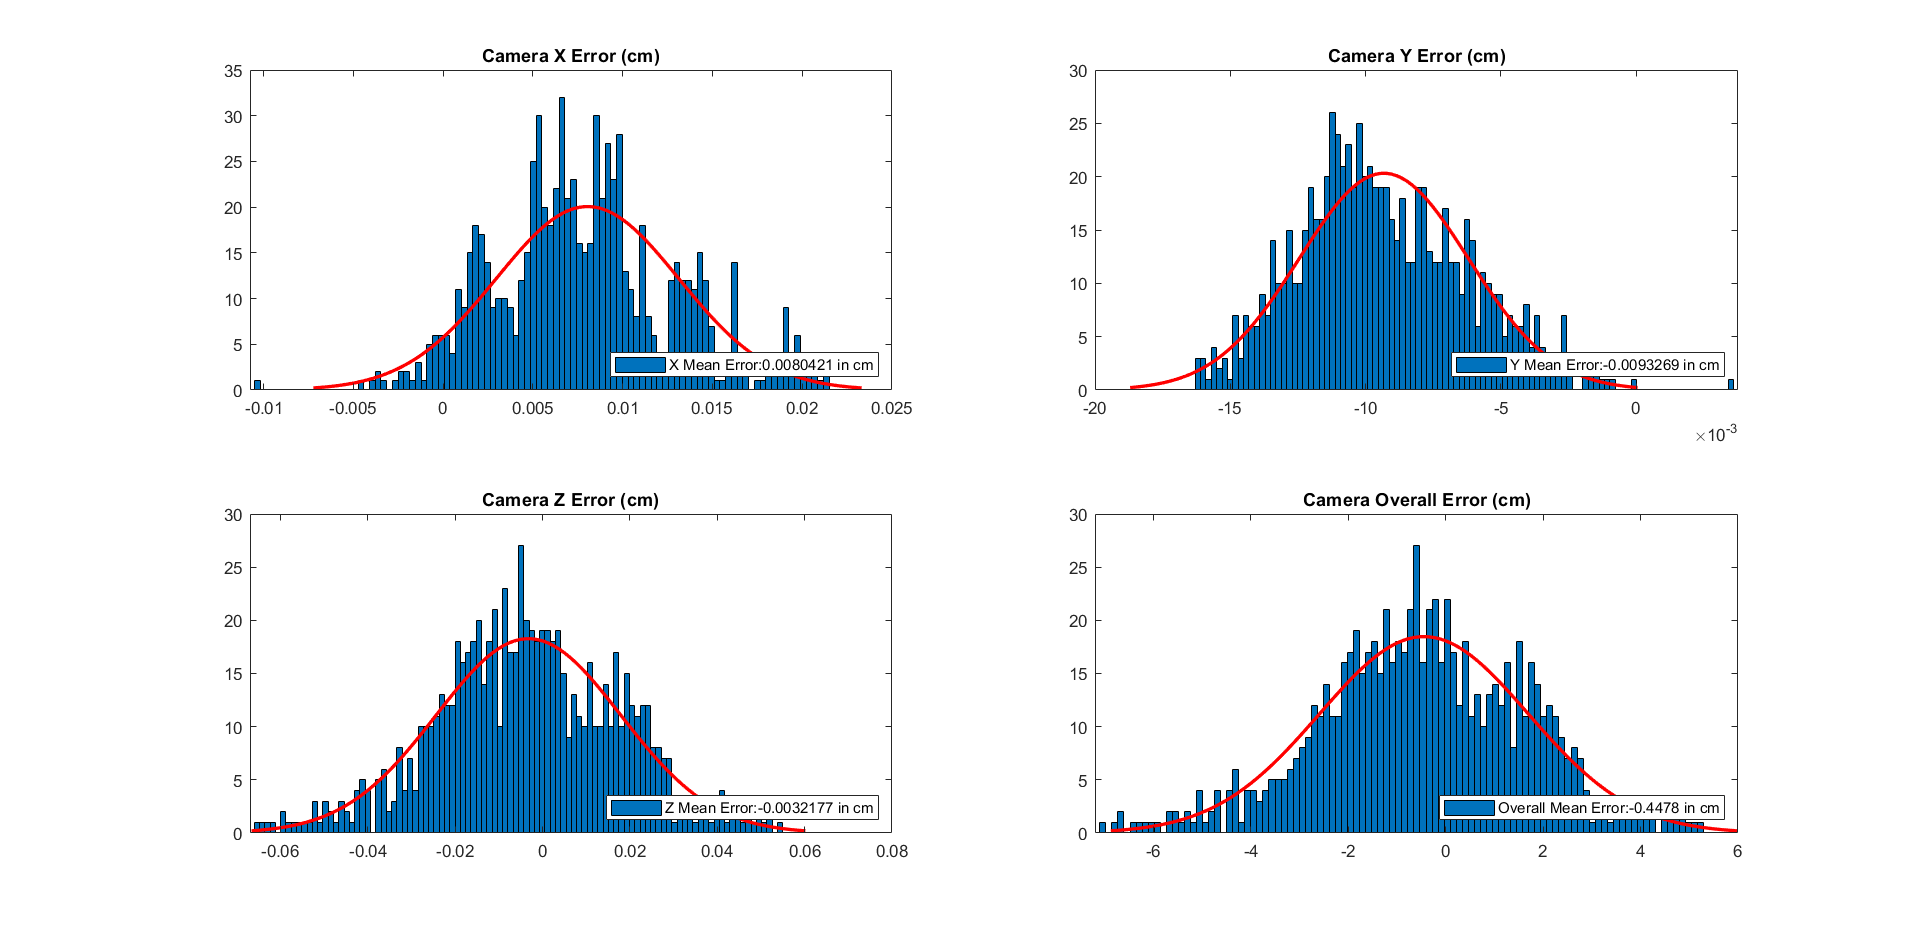
\includegraphics[scale= 0.3]{Images/Cam_intrinsic.png}
    \caption{Camera Intrinsic Calibration to find standard measurement error}
    \label{camintrinsic2}
\end{figure}

\subsection{LiDAR Intrinsic Calibration}
Intrinsic calibration of LiDAR was performed by using twenty-five images of checkered board pattern by positioning checkered board at various location w.r.t LiDAR. Similar to the stereo camera, the ground truth and measurement data of LiDAR were generated. Finally, these two datasets were used to find the standard measurement error of LiDAR. The histogram of LiDAR calibration errors is pictured in Fig. \ref{lidarintrinsic}.

\begin{figure}
    \centering
    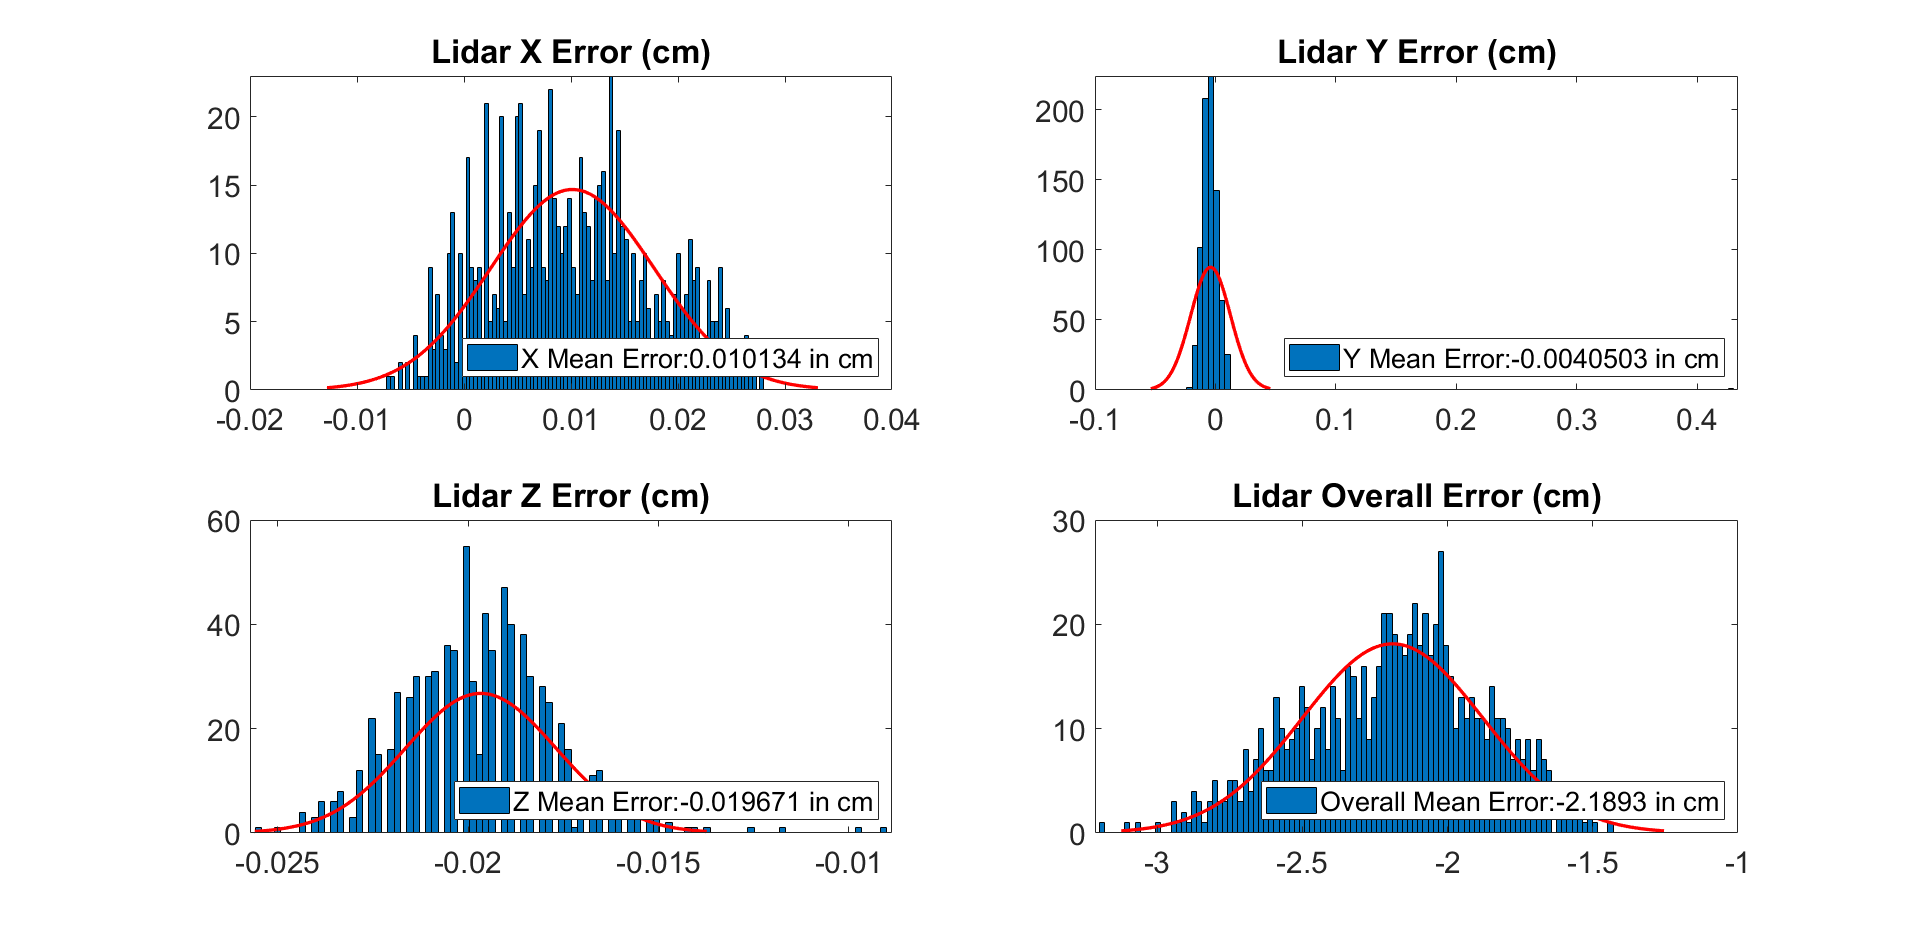
\includegraphics[scale= 0.3]{Images/Lidar_Intrinsic.png}
    \caption{LiDAR Intrinsic Calibration to find standard measurement error}
    \label{lidarintrinsic}
\end{figure}

\subsection{Stereo camera and LiDAR Extrinsic Calibration}
In the Extrinsic calibration for both sensors, the same data as in intrinsic calibration was used to get a 3-D rigid transformation matrix. The data set collected manually is considered as ground truth data. The 3-D transformation matrix is derived from both the ground truth data. There is a total of two transformation matrices that can be derived, for Camera to LiDAR transformation and LiDAR to camera transformation. After, the measurement data set was generated using transformation matrices. Further ground truth and measurement data set were used to derive standard measurement error for 3-D rigid transformation. The transformation error is mentioned in table \ref{Extrinsics} and the histogram is shown in Fig. \ref{lExtrinsic}.        

\begin{figure}
    \centering
    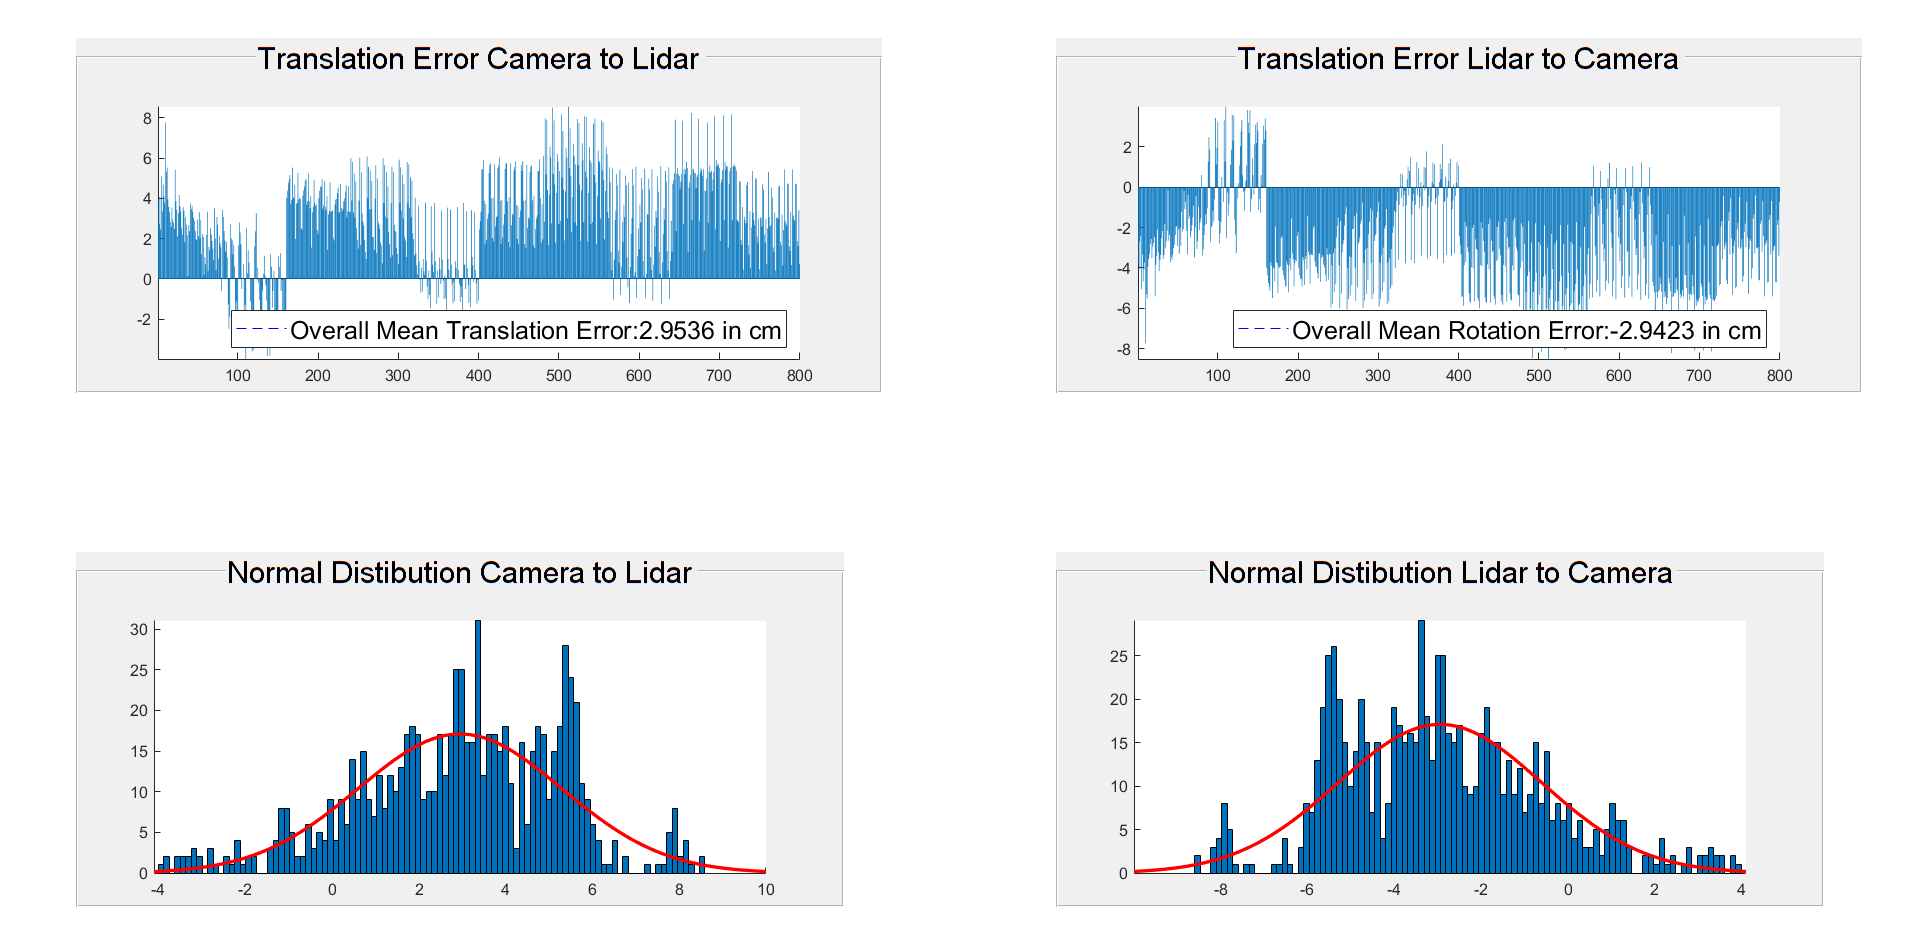
\includegraphics[scale= 0.27]{Images/Extrinsic_Calibration.png}
    \caption{Stereo Camera and LiDAR Extrinsic Calibration}
    \label{lExtrinsic}
\end{figure}

\begin{table}
    \centering
    \begin{tabular}{|l|c|c|}
        \hline
        Description & Camera to LiDAR & LiDAR to Camera \\
        \hline
        Re-projection Error & 29.5 mm & -29.42 mm \\
        \hline
    \end{tabular}
    \caption{Re-projection Error of Extrinsic Calibration}
    \label{Extrinsics}
\end{table}

\section{Object Detection}
Any object in this world has special features that make it stand different from others, three edges for a triangle for instance. Such features can be used to classify different objects. However, object detection is not just a task of classifying the object, it also includes object classification, localization, and mapping w.r.t body frame. There are many computer vision techniques for object detection. However, such an algorithm might require a controlled environment. For instance, the image thresholding technique needs an indoor environment without sunlight. Therefore, This helps to reduce real-time challenges faced in the object detection algorithms.

\textbf{1. Occlusion:}
This problem occurs when one object obstructs the view of another object that is behind it. In such a condition, the computer program does not completely understand the features of the object or fail to recognize the occluded object and gives the combined detection result which is not acceptable in a real-world application. 

\textbf{2. Change of viewpoint:}
Non-homogeneous 3D objects with complex shapes may not be recognized when viewed from another direction than the one for which the algorithm developed for. For example, for a case of detecting a person, if the detector's viewpoint is changed from front to right then the algorithm may detect fewer features of the person, and or it may fail to detect the person. 

\textbf{3. Variation in size:}
The algorithms are developed to work in real-time object detection applications. Thus, images with small sizes are used in such object detection tasks to overcome the computational load. Therefore, this makes recognition very difficult for the objects occupying few pixels in the image. In such a case, the object detection algorithm is effective only for a limited range.  

\textbf{4. Motion Blur:}
When it is a case of detecting a moving object such as a car or any vehicle, it is usually the issue that the camera image is blurred because of the slow shutter speed. In such a scenario, robust object detectors are recommended to use.


\begin{figure}
    \centering
    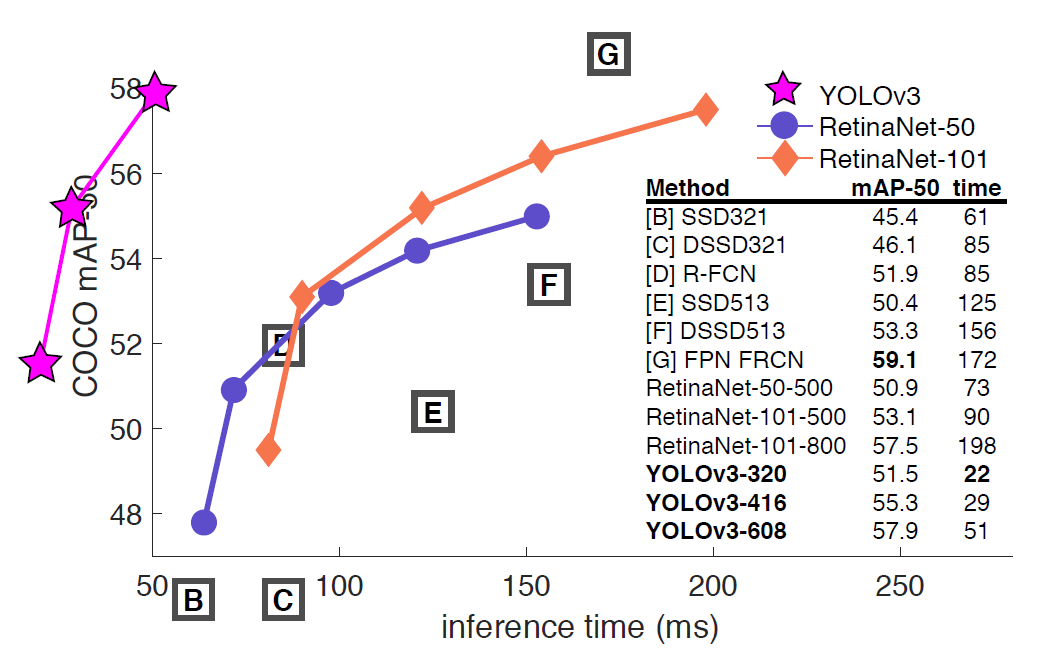
\includegraphics[scale= 0.35]{Images/yolov3time.png}
    \caption{Performance of YOLO-v3 compare to Other Neural Networks \cite{yolov3}}
    \label{yolov3time}
\end{figure}

\subsection{Detect Object in Stereo Camera using Deep Learning}
Object detection using deep learning techniques work faster than other machine learning algorithm and provide an accurate prediction of object class and location within the image frame. Neural network learns features of objects while training and store them as weights and biases of the network. In this research work, the YOLO (you only look once) neural network was used to detect four classes of geometric shapes like pyramid, square, cone, and cylinder. This network was trained on self-generated training data set of 11000 images of mentioned classes of objects.   

YOLO-v3 neural network is proven to be faster than other deep learning techniques as seen in Fig. \ref{yolov3time}. This is because unlike a traditional search algorithm it divides the input image into grids to perform a search of objects. The incredible processing speed of YOLO has made it qualify for real-time object detection applications.

\begin{figure}
    \centering
    \includegraphics[scale= 0.35]{Images/LiDARlabel.png}
    \caption{Data Pipeline to Generate LiDAR Label using Camera Data \cite{MATLAB_Lidar}}
    \label{lidarlabel}
\end{figure}

\subsection{Detect Object in LiDAR using Image Label}
To use an individual neural network for object detection from LiDAR data consumes a lot of processing time. Instead, using the labels generated from image data to predict a 3-D bounding box in LiDAR data costs less time. A schematic of the data pipeline to predict a 3-D bounding box in LiDAR data using Image label is given in Fig. \ref{lidarlabel}.     

